Para experimentar con las herramientas desarolladas, realizamos traceroutes a IPs pertenecientes a sitios web de universidades en diferentes paises alrededor del mundo. De todas las epxerimentaciones que hicimos nos quedamos con tres universidades:
\begin{itemize}
  \item Lomonosov Moscu State University, situada en Moscu, Rusia, Europa. (\url{www.msu.ru})
  \item The University of Tokyo, situada en Tokio, Japon, Asia. (\url{www.u-tokyo.ac.jp})
  \item The University of Sydney, situada en Sydney, Australia, Oceania. (\url{www.sydney.edu.au})
\end{itemize}

\subsection{Lomonosov Moscu State University}
A continuación podemos observar los resultados que obtuvimos al probar nuestra herramiento de traceroute
con destino la universidad situada en Moscu, es decir \url{www.msu.ru}.

\begin{figure}[H]
\begin{center}
\begin{tabular}{|c|c|c|c|c|}
  \hline
  HOP & RTT & RTT RELATIVO & Ubicación & ZRTT \\ \hline
 192.168.1.1 & 66 ms & 0 & - & -0,2714373843 \\ \hline
 10.21.192.1 & 75 ms & 9 & - & -0,160394818 \\ \hline
 10.242.1.17 & 80 ms & 5 & - & -0,2097470697 \\ \hline
 208.178.195.210 & 84 ms & 4 & (Estados Unidos) & -0,2220851326 \\ \hline
 208.178.195.209 & 91 ms & 7 & (Estados Unidos) & -0,1850709439 \\ \hline
 * & & & & \\ \hline
 4.69.158.253 & 335 ms & \textbf{244} & Suecia & \textbf{2,739049969} \\ \hline
 4.69.158.253 & 329 ms & -6 & Suecia & -0,3454657619 \\ \hline
 213.242.110.198 & 356 ms & 27 & (Reino Unido) & 0,06169031462 \\ \hline
 * & & & & \\ \hline
 194.85.40.229 & 462 ms & 106 & (Rusia) & 1,036397286 \\ \hline
 194.190.254.118 & 378 ms & -84 & (Rusia) & -1,30783467 \\ \hline
 93.180.0.172 & 464 ms & 86 & Moscu (Rusia) & 0,7896360271 \\ \hline
 188.44.33.30 & 439 ms & -25 & Moscu (Rusia) & -0,5798889574 \\ \hline
 188.44.33.2 & 365 ms & -74 & Moscu (Rusia) & -1,184454041 \\ \hline
 188.44.50.103 & 383 ms & 18 & Moscu (Rusia) & -0,0493522517 \\ \hline
% \hline
%  & Average: & 22 & & & \\
%  & Std Deviation: & 81.0555365166 & & & \\
%  & Outlier: & 4.69.158.253 & & & \\
% \hline

\end{tabular}


Además obtuvimos mediante la técnica de estimación de outliers el salto desde Estados Unidos (208.178.195.209) hacia Suecia (4.69.158.253). Efectivamente ese es un salto transcontinental. 
En el siguiente gráfico podemos observar las variaciones de ZRTT a lo largo de los saltos de la ruta:


\caption{Tabla generada por Traceroute a la Universidad de Moscu (188.44.50.103)}
% \label{my-label}
\end{center}
\end{figure}

Podemos observar en el gráfico que además del salto identificado mediante la técnica de Cimbala, sobresalen también el salto desde el Reino Unido hasta Rusia. Aquí se observa la ventaja de este método gráfico y la efectividad del método de Cimbala. 

\begin{center}
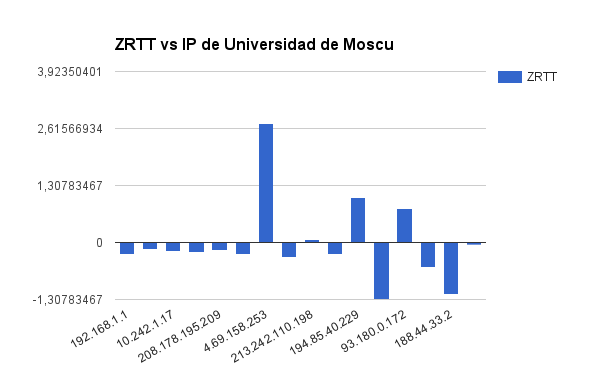
\includegraphics[width=\textwidth]{imgs/moscu.png}
\end{center}


\subsection{The University of Tokyo}
Acontinuación mostramos los resultados obtenidos cuando tomamos como destino la
Universidad de Tokio, es decir \url{www.u-tokyo.ac.jp}.

\begin{figure}[H]
\begin{center}
\begin{tabular}{|c|c|c|c|c|}
  \hline
  HOP & RTT & RTT RELATIVO & Ubicación & ZRTT \\ \hline
  192.168.1.1 & 62 ms & 0 & - & -0,3018867925 \\ \hline
  10.21.192.1 & 159 ms &  97  & - &  1,528301887 \\ \hline
  10.242.1.17 & 123 ms &  -36 & - & -0,9811320755 \\ \hline
  195.22.220.33 & 76 ms & -47 & (Italia) & -1,188679245 \\ \hline
  195.22.220.32 & 127 ms &  51  & (Italia)&  0,6603773585 \\ \hline
  195.22.219.145 &  160 ms &  33  & (Italia)&  0,320754717 \\ \hline
  195.22.219.145 &  95 ms & -65 & (Italia) & -1,528301887 \\ \hline
  149.3.181.65 &  106 ms &  11  & (Italia) & -0,09433962264 \\ \hline
  129.250.2.227 & 222 ms &  116 & Englewood (Estados Unidos)&  1,886792453 \\ \hline
  129.250.4.13 &  272 ms &  50  & Englewood (Estados Unidos)&  0,641509434 \\ \hline
  129.250.2.54 &  269 ms &  -3  & Englewood (Estados Unidos) & -0,358490566 \\ \hline
  129.250.3.86 &  418 ms &  \textbf{149} & Englewood (Estados Unidos)&  \textbf{2,509433962} \\ \hline
  129.250.6.188 & 405 ms &  -13 & Englewood (Estados Unidos) & -0,5471698113 \\ \hline
  129.250.2.255 & 404 ms &  -1  & Englewood (Estados Unidos) & -0,320754717 \\ \hline
  61.200.80.218 & 396 ms &  -8  & (Japón) & -0,4528301887 \\ \hline
  158.205.192.173 & 414 ms &  18  & (Japón)&  0,03773584906 \\ \hline
  158.205.192.86 &  413 ms &  -1  & (Japón) & -0,320754717 \\ \hline
  158.205.121.250 & 387 ms &  -26 & (Japón) & -0,7924528302 \\ \hline
  154.34.240.254 &  407 ms &  20  & (Japón)&  0,07547169811 \\ \hline
  210.152.135.178 & 399 ms &  -8  & (Japón) & -0,4528301887 \\ \hline
\end{tabular}
\caption{Tabla generada por Traceroute a la Universidad de Tokyo (210.152.135.178)}
% \label{my-label}
\end{center}
\end{figure}


\begin{center}
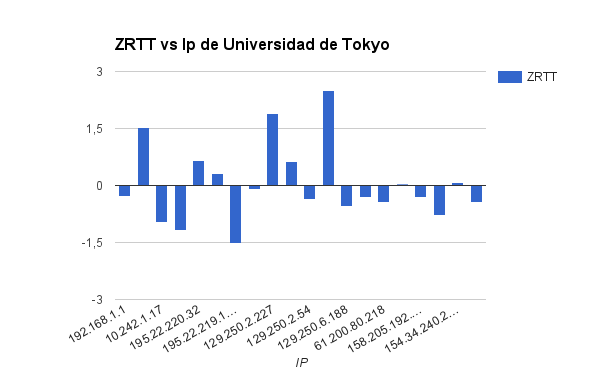
\includegraphics[width=\textwidth]{imgs/tokyo.png}
\end{center}


\subsection{The University of Sydney}
A continuacion podemos observar los resultados que obtuvimos al probar nuestra herramiento de traceroute
con destino \url{www.sydney.edu.au}.

\begin{figure}[H]
\begin{center}
\begin{tabular}{|c|c|c|c|c|}
  \hline
  HOP & RTT & RTT RELATIVO & Ubicación & ZRTT \\ \hline
  192.168.1.1     & 83 ms  & 0          & Argentina & -0,3940627873 \\ \hline
  10.21.192.1     & 167 ms & 84         & Argentina & 0,7093130172  \\ \hline
  10.242.1.17     & 83 ms  & -84        & Argentina & -1,497438592  \\ \hline
  195.22.220.33   & 67 ms  & -16        & Italia & -0,6042296073 \\ \hline
  195.22.220.32   & 78 ms  & 11         & Italia & -0,2495730986 \\ \hline
  195.22.206.190  & 270 ms & \textbf{192}        &Italia - & \textbf{2,127939052}   \\ \hline
  198.32.176.177  & 312 ms & 42         &Redwood City (Estados Unidos) - & 0,1576251149  \\ \hline
  202.158.194.176 & 419 ms & 107        &Canberra (Australia) - & 1,011427821   \\ \hline
  113.197.15.146  & 458 ms & 39         &Canberra (Australia) - & 0,1182188362  \\ \hline
  138.44.5.47     & 416 ms & -42        &Canberra (Australia) - & -0,9457506896 \\ \hline
  * * *           &        &            & - & -0,3940627873 \\ \hline
  * * *           &        &            & - & -0,3940627873 \\ \hline
  129.78.5.8      & 413 ms & -3         &Sydney (Australia) & -0,4334690661 \\ \hline
\end{tabular}
\caption{Tabla generada por Traceroute a la Universidad de Sydney (129.78.5.8)}
% \label{my-label}
\end{center}
\end{figure}




\begin{center}
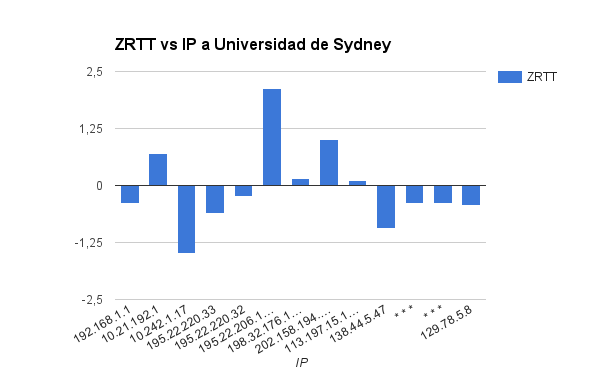
\includegraphics[width=\textwidth]{imgs/sydney.png}
\end{center}




